\section{Crypto Proxy}
This exercice proposes the creation of a crypto proxy. To connect to a server we would usually create a raw tcp socket and send information through it. 

We are going to implement a TCP proxy that acts in between the sockets, and encrypts the information passed through it.

\begin{figure}[htb]
	\begin{centering}
		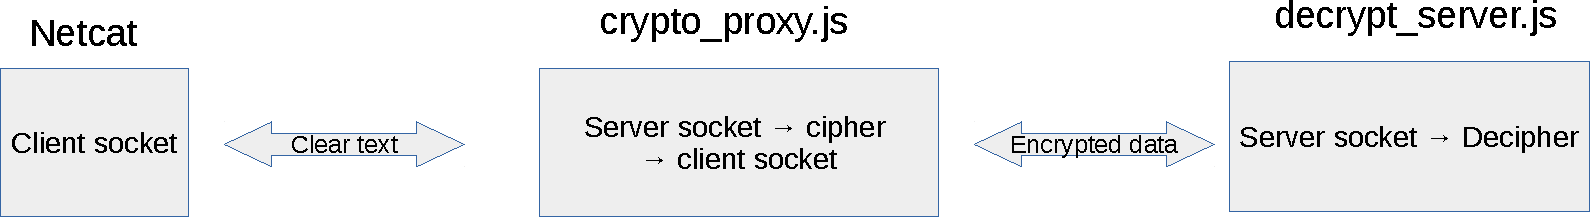
\includegraphics[width=0.7\columnwidth]{\securitydir/basicJsCrypto/figures/crypto_proxy}
		\par\end{centering}
	\caption{\label{fig:crypto_proxy} Connection scheme}
\end{figure}


For the first socket (local socket), we are going to use netcat. netcat allows to create a TCP socket easily from the CLI. In the real world, netcat would be much more complex program.

The second socket will recieve the unencrypted data, cipher it using AES 256 and resend it to the server.

Finally, the remote socket recieves the encrypted data, and deciphers it. In our implementation, the server saves the data into a file.

To run the experiment we are going to need three different terminals.

\begin{lstlisting}[style=terms]
$ nodejs decrypt_server.js
$ nodejs crypto_proxy.js
$ nc localhost 1234
\end{lstlisting}


If we use wireshark we can see that the first connection is in clear text, while the second isnt.

For the next part, we are going to send a picture through the proxy. To do this, execute netcat with a pipe where Tux.png is the picture to send.

\begin{lstlisting}[style=terms]
$ cat Tux.png | nc localhost 1234
\end{lstlisting}

If all goes well, we shall see a picture named test.png, that should be the same as Tux.png

If we capture this traffic with wireshark, then select the option "Follow TCP Stream" on any tcp packet, and finally select "Save as..." we can capture files directly from wireshark. If we do this with the connection that isn't encrypted, we can save the picture, while if we do this in the connection that isn't, we are getting pseudonoise. This is a very powerful tool, as we can see and save any non-encrypted traffic that goes trough our computer (Now imagine you are the gateway in a public wifi).

\subsection{Exercises}
\begin{enumerate}
	\item Write the decrypt server. It must receive the data from the socket, pipe it through a AES decipher and then save it to a file.
	
	\item Write the proxy server. It should have two different sockets. One that works as a server en receives the data from the netcat, and the other must be a client that connects to the decrypt\_server. The data received from the netcat should be encrypted and then sent to the decrypt server.
	
	\item Improve the proxy and the server so full duplex encrypted conection is possible.
\end{enumerate}

\begin{js}
//crypto proxy.js
const net = require('net');
const crypto = require('crypto');

// tunnel entrance

password = '01234567';

// this socket will connect to the decrypt server
destination = new net.Socket();
destination.connect(5678, 'localhost');
// this object works as Stream, encrypting the data dat goes through it
cipher = crypto.createCipher('aes-256-ecb', password);

// we create the server that listens to connections
source = net.createServer(function (socket) {
    // the output of the listening socket is piped to the cipher input, and the output of the cipher is sent to the server.
    socket.pipe(cipher).pipe(destination);
}).listen(1234);
\end{js}


\begin{js}
// decrypt server.js
const net = require('net');
const crypto = require('crypto');
const fs = require('fs');

// tunnel exit
var wstream = fs.createWriteStream('test.png');

password = '01234567';

cipher = crypto.createDecipher('aes-256-ecb', password);

net.createServer(function (sock) {
    sock.pipe(cipher).pipe(wstream);

    sock.on('close', function (data) {
        wstream.end();
        console.log("Message received.")
    });
}).listen(5678);
\end{js}
